\documentclass[ngerman]{report}
\usepackage[T1]{fontenc}
\usepackage[ngerman]{babel}
\usepackage{parskip} %Einrückung neuer Paragraphen verhindern
\usepackage{booktabs}%Tabellenlinien etc.

\usepackage{amssymb, amsmath}
\newcommand{\myvec}[1]{\ensuremath{\begin{pmatrix}#1\end{pmatrix}}}
\usepackage{bm}

\usepackage{tikz}
\usetikzlibrary {arrows.meta, calc}
\usepackage{pdfpages}

\usepackage{hyperref}
\usepackage{cleveref}
\hypersetup{hidelinks}

\title{\textbf{R}echner\textbf{U}nterstütztes\textbf{Z}eichnen RUZ\\Technische Spezifikationen}
\author{Ansgar Rütten}
\date{09. März 2024\\Stand:\today}


\begin{document}
\maketitle
\newpage
\tableofcontents
\newpage
\chapter{Elemente der Zeichnung}

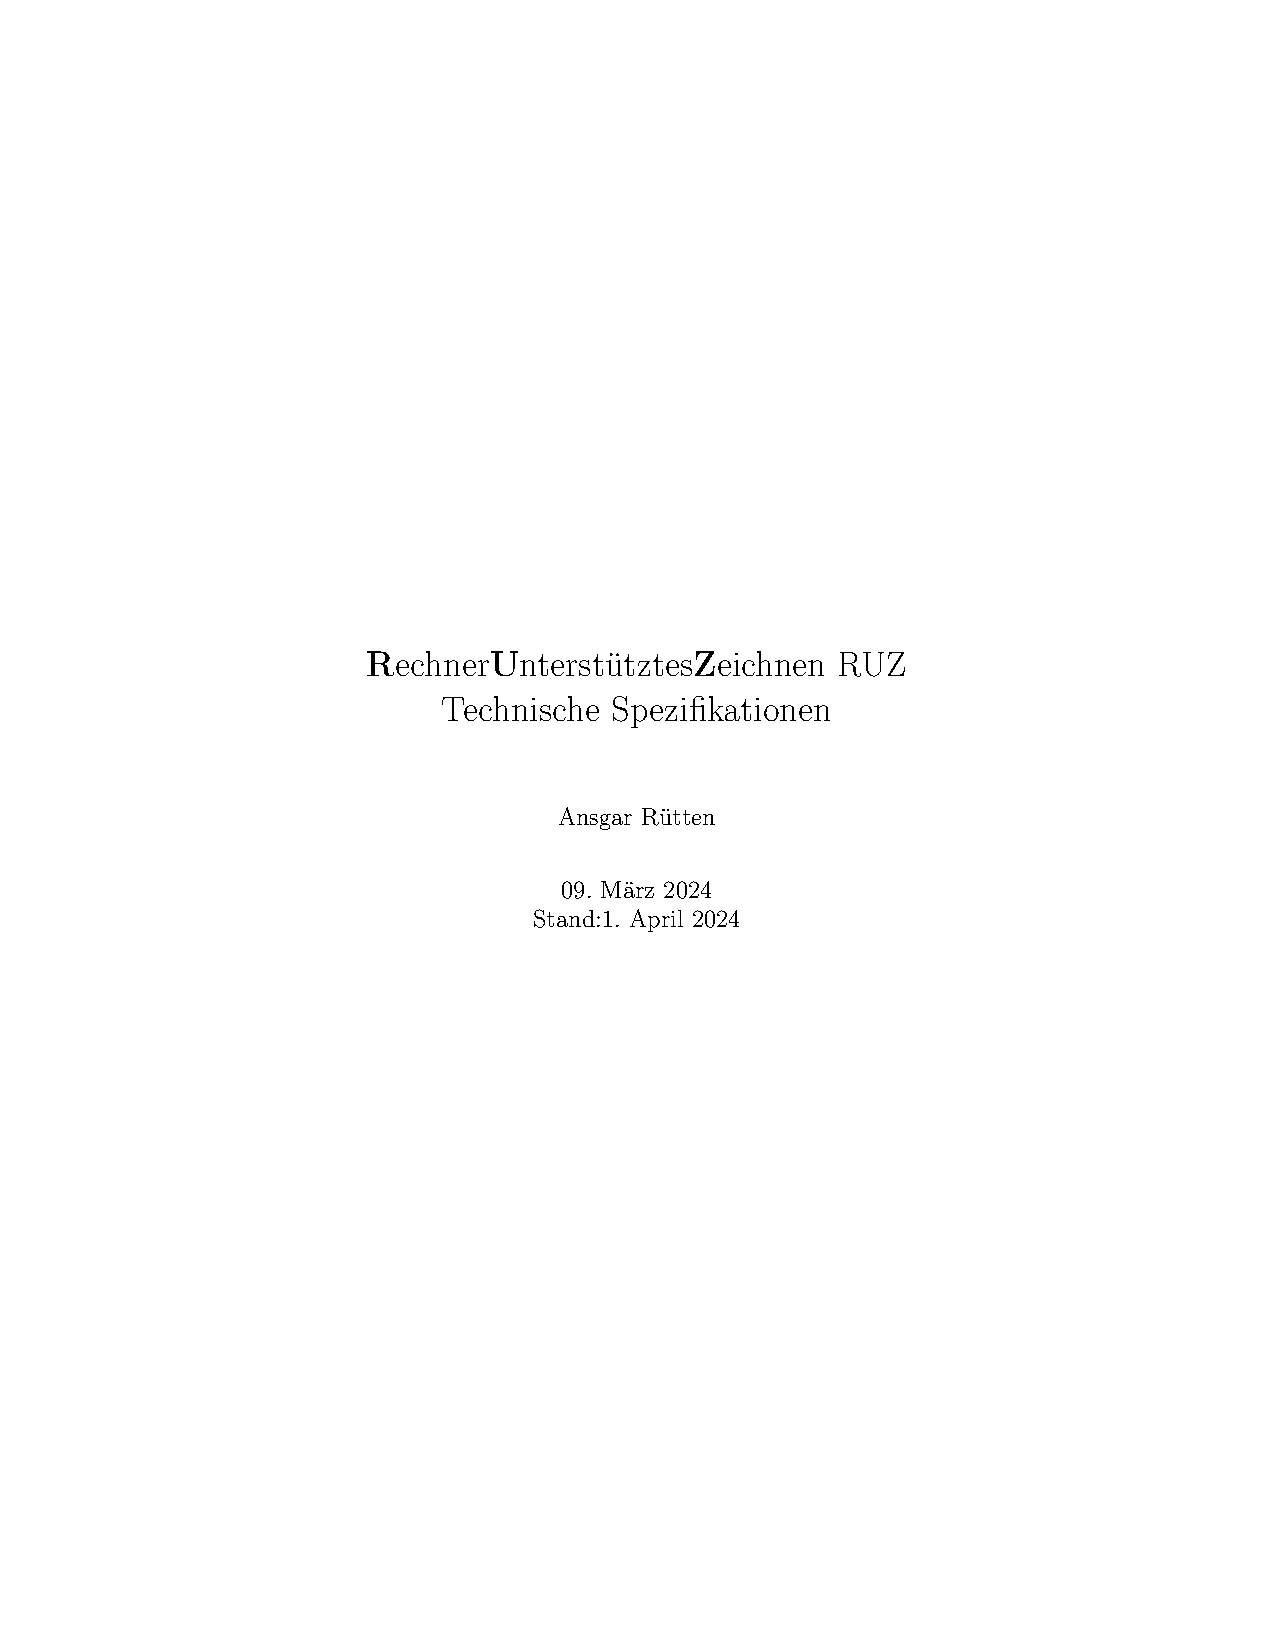
\includepdf[
	pages=-
	addtotoc={	
	}
]{Test/Untertest/Neues_Text_d_ok_ument.pdf}

\end{document}